% Options for packages loaded elsewhere
\PassOptionsToPackage{unicode}{hyperref}
\PassOptionsToPackage{hyphens}{url}
\documentclass[
  ignorenonframetext,
]{beamer}
\newif\ifbibliography
\usepackage{pgfpages}
\setbeamertemplate{caption}[numbered]
\setbeamertemplate{caption label separator}{: }
\setbeamercolor{caption name}{fg=normal text.fg}
\beamertemplatenavigationsymbolsempty
% remove section numbering
\setbeamertemplate{part page}{
  \centering
  \begin{beamercolorbox}[sep=16pt,center]{part title}
    \usebeamerfont{part title}\insertpart\par
  \end{beamercolorbox}
}
\setbeamertemplate{section page}{
  \centering
  \begin{beamercolorbox}[sep=12pt,center]{section title}
    \usebeamerfont{section title}\insertsection\par
  \end{beamercolorbox}
}
\setbeamertemplate{subsection page}{
  \centering
  \begin{beamercolorbox}[sep=8pt,center]{subsection title}
    \usebeamerfont{subsection title}\insertsubsection\par
  \end{beamercolorbox}
}
% Prevent slide breaks in the middle of a paragraph
\widowpenalties 1 10000
\raggedbottom
\AtBeginPart{
  \frame{\partpage}
}
\AtBeginSection{
  \ifbibliography
  \else
    \frame{\sectionpage}
  \fi
}
\AtBeginSubsection{
  \frame{\subsectionpage}
}
\usepackage{iftex}
\ifPDFTeX
  \usepackage[T1]{fontenc}
  \usepackage[utf8]{inputenc}
  \usepackage{textcomp} % provide euro and other symbols
\else % if luatex or xetex
  \usepackage{unicode-math} % this also loads fontspec
  \defaultfontfeatures{Scale=MatchLowercase}
  \defaultfontfeatures[\rmfamily]{Ligatures=TeX,Scale=1}
\fi
\usepackage{lmodern}
\usetheme[]{Madrid}
\usecolortheme[]{dolphin}
\ifPDFTeX\else
  % xetex/luatex font selection
\fi
% Use upquote if available, for straight quotes in verbatim environments
\IfFileExists{upquote.sty}{\usepackage{upquote}}{}
\IfFileExists{microtype.sty}{% use microtype if available
  \usepackage[]{microtype}
  \UseMicrotypeSet[protrusion]{basicmath} % disable protrusion for tt fonts
}{}
\makeatletter
\@ifundefined{KOMAClassName}{% if non-KOMA class
  \IfFileExists{parskip.sty}{%
    \usepackage{parskip}
  }{% else
    \setlength{\parindent}{0pt}
    \setlength{\parskip}{6pt plus 2pt minus 1pt}}
}{% if KOMA class
  \KOMAoptions{parskip=half}}
\makeatother
\usepackage{color}
\usepackage{fancyvrb}
\newcommand{\VerbBar}{|}
\newcommand{\VERB}{\Verb[commandchars=\\\{\}]}
\DefineVerbatimEnvironment{Highlighting}{Verbatim}{commandchars=\\\{\}}
% Add ',fontsize=\small' for more characters per line
\usepackage{framed}
\definecolor{shadecolor}{RGB}{248,248,248}
\newenvironment{Shaded}{\begin{snugshade}}{\end{snugshade}}
\newcommand{\AlertTok}[1]{\textcolor[rgb]{0.94,0.16,0.16}{#1}}
\newcommand{\AnnotationTok}[1]{\textcolor[rgb]{0.56,0.35,0.01}{\textbf{\textit{#1}}}}
\newcommand{\AttributeTok}[1]{\textcolor[rgb]{0.13,0.29,0.53}{#1}}
\newcommand{\BaseNTok}[1]{\textcolor[rgb]{0.00,0.00,0.81}{#1}}
\newcommand{\BuiltInTok}[1]{#1}
\newcommand{\CharTok}[1]{\textcolor[rgb]{0.31,0.60,0.02}{#1}}
\newcommand{\CommentTok}[1]{\textcolor[rgb]{0.56,0.35,0.01}{\textit{#1}}}
\newcommand{\CommentVarTok}[1]{\textcolor[rgb]{0.56,0.35,0.01}{\textbf{\textit{#1}}}}
\newcommand{\ConstantTok}[1]{\textcolor[rgb]{0.56,0.35,0.01}{#1}}
\newcommand{\ControlFlowTok}[1]{\textcolor[rgb]{0.13,0.29,0.53}{\textbf{#1}}}
\newcommand{\DataTypeTok}[1]{\textcolor[rgb]{0.13,0.29,0.53}{#1}}
\newcommand{\DecValTok}[1]{\textcolor[rgb]{0.00,0.00,0.81}{#1}}
\newcommand{\DocumentationTok}[1]{\textcolor[rgb]{0.56,0.35,0.01}{\textbf{\textit{#1}}}}
\newcommand{\ErrorTok}[1]{\textcolor[rgb]{0.64,0.00,0.00}{\textbf{#1}}}
\newcommand{\ExtensionTok}[1]{#1}
\newcommand{\FloatTok}[1]{\textcolor[rgb]{0.00,0.00,0.81}{#1}}
\newcommand{\FunctionTok}[1]{\textcolor[rgb]{0.13,0.29,0.53}{\textbf{#1}}}
\newcommand{\ImportTok}[1]{#1}
\newcommand{\InformationTok}[1]{\textcolor[rgb]{0.56,0.35,0.01}{\textbf{\textit{#1}}}}
\newcommand{\KeywordTok}[1]{\textcolor[rgb]{0.13,0.29,0.53}{\textbf{#1}}}
\newcommand{\NormalTok}[1]{#1}
\newcommand{\OperatorTok}[1]{\textcolor[rgb]{0.81,0.36,0.00}{\textbf{#1}}}
\newcommand{\OtherTok}[1]{\textcolor[rgb]{0.56,0.35,0.01}{#1}}
\newcommand{\PreprocessorTok}[1]{\textcolor[rgb]{0.56,0.35,0.01}{\textit{#1}}}
\newcommand{\RegionMarkerTok}[1]{#1}
\newcommand{\SpecialCharTok}[1]{\textcolor[rgb]{0.81,0.36,0.00}{\textbf{#1}}}
\newcommand{\SpecialStringTok}[1]{\textcolor[rgb]{0.31,0.60,0.02}{#1}}
\newcommand{\StringTok}[1]{\textcolor[rgb]{0.31,0.60,0.02}{#1}}
\newcommand{\VariableTok}[1]{\textcolor[rgb]{0.00,0.00,0.00}{#1}}
\newcommand{\VerbatimStringTok}[1]{\textcolor[rgb]{0.31,0.60,0.02}{#1}}
\newcommand{\WarningTok}[1]{\textcolor[rgb]{0.56,0.35,0.01}{\textbf{\textit{#1}}}}
\usepackage{graphicx}
\makeatletter
\newsavebox\pandoc@box
\newcommand*\pandocbounded[1]{% scales image to fit in text height/width
  \sbox\pandoc@box{#1}%
  \Gscale@div\@tempa{\textheight}{\dimexpr\ht\pandoc@box+\dp\pandoc@box\relax}%
  \Gscale@div\@tempb{\linewidth}{\wd\pandoc@box}%
  \ifdim\@tempb\p@<\@tempa\p@\let\@tempa\@tempb\fi% select the smaller of both
  \ifdim\@tempa\p@<\p@\scalebox{\@tempa}{\usebox\pandoc@box}%
  \else\usebox{\pandoc@box}%
  \fi%
}
% Set default figure placement to htbp
\def\fps@figure{htbp}
\makeatother
\setlength{\emergencystretch}{3em} % prevent overfull lines
\providecommand{\tightlist}{%
  \setlength{\itemsep}{0pt}\setlength{\parskip}{0pt}}
\usepackage{bookmark}
\IfFileExists{xurl.sty}{\usepackage{xurl}}{} % add URL line breaks if available
\urlstyle{same}
\hypersetup{
  pdftitle={Module 5: Simulations and Parallel Computing},
  pdfauthor={Benjamin Smith},
  hidelinks,
  pdfcreator={LaTeX via pandoc}}

\title{\texorpdfstring{Module 5: Simulations and Parallel
Computing}{Module 5: Simulations and Parallel Computing}}
\author{\texorpdfstring{Benjamin Smith}{Benjamin Smith}}
\date{07/21/2026}

\begin{document}
\frame{\titlepage}

\begin{frame}{Outline}
\protect\phantomsection\label{outline}
In this module, we will review

\begin{itemize}
\tightlist
\item
  Simulation Study
\item
  Rationale for Simulations
\item
  Parallel Computing in R
\end{itemize}
\end{frame}

\begin{frame}{Simulation study}
\protect\phantomsection\label{simulation-study}
\begin{itemize}
\item
  Simulation: A numerical techniques for conducting experiments on the
  computer
\item
  Monte Carlo simulation: Computer experiment involving random sampling
  from probability distributions
\end{itemize}
\end{frame}

\begin{frame}{Why simulation?}
\protect\phantomsection\label{why-simulation}
To establish/validate the properties of statistical methods

\begin{itemize}
\tightlist
\item
  Exact analytical derivations of properties are \textbf{rarely}
  possible
\item
  Large sample approximations to properties are \textbf{often possible},
  but need to evaluate their relevance to (finite) sample sizes likely
  to be encountered in practice
\end{itemize}

\pause

Moreover, analytical results may require \textbf{assumptions} (e.g.,
normality)

\begin{itemize}
\tightlist
\item
  But what happens when these assumptions are violated?
\item
  Analytical results, even large sample ones, may not be possible
\end{itemize}
\end{frame}

\begin{frame}{Considerations for simulation}
\protect\phantomsection\label{considerations-for-simulation}
\begin{itemize}
\tightlist
\item
  Is an estimator \textbf{biased} in finite samples? Is it still
  \textbf{consistent} under departures from assumptions? What is its
  \textbf{sampling variance}?
\item
  How does it \textbf{compare} to competing estimators on the basis of
  bias, precision, etc.? \pause
\item
  Does a procedure for constructing a \textbf{confidence interval} for a
  parameter achieve the advertised \textbf{nominal level of coverage}?
\item
  Does a \textbf{hypothesis testing} procedure attain the advertised
  \textbf{level} or \textbf{size}?
\item
  If it does, what \textbf{power} is possible against different
  alternatives to the null hypothesis? Do different test procedures
  deliver different power?
\end{itemize}
\end{frame}

\begin{frame}{Monte Carlo simulation}
\protect\phantomsection\label{monte-carlo-simulation}
\begin{itemize}
\tightlist
\item
  Generate \(S\) independent data sets under the conditions of interest
\item
  Compute the numerical value of the estimator/test statistic \(T\)
  (data) for each data set \(\Rightarrow T_{1}, \ldots, T_{S}\)
\item
  If \(S\) is large enough, \textbf{summary statistics} across
  \(T_{1}, \ldots, T_{S}\) should be good \textbf{approximations} to the
  true sampling properties of the estimator/test statistic under the
  conditions of interest
\end{itemize}
\end{frame}

\begin{frame}{Simulations for properties of estimators}
\protect\phantomsection\label{simulations-for-properties-of-estimators}
Example: Compare 3 estimators for the \textbf{mean} \(\mu\) of a
distribution based on i.i.d. draws \(Y_{1}, \ldots, Y_{n}\)

\begin{itemize}
\tightlist
\item
  Sample mean \(T^{(1)}\)
\item
  Sample 20\% trimmed mean \(T^{(2)}\)
\item
  Sample median \(T^{(3)}\)
\end{itemize}
\end{frame}

\begin{frame}{Simulations for properties of estimators (cont'd)}
\protect\phantomsection\label{simulations-for-properties-of-estimators-contd}
\textbf{Simulation procedure}: For a particular choice of \(\mu, n\),
and true underlying distribution

\begin{itemize}
\item
  Generate independent draws \(Y_{1}, \ldots, Y_{n}\) from the
  distribution
\item
  Compute \(T^{(1)}, T^{(2)}, T^{(3)}\)
\item
  Repeat \(S\) times
  \(T_{1}^{(1)}, \ldots, T_{S}^{(1)} ; \quad T_{1}^{(2)}, \ldots, T_{S}^{(2)} ; \quad T_{1}^{(3)}, \ldots, T_{S}^{(3)}\)
\item
  Compute for \(k=1,2,3\) \[
  \widehat{\mu}=S^{-1} \sum_{s=1}^{S} T_{s}^{(k)}=\bar{T}^{(k)}, \widehat{\text { bias }}=\bar{T}^{(k)}-\mu
  \]
\end{itemize}

\[
\widehat{\sigma}=\sqrt{(S-1)^{-1} \sum_{s=1}^{S}\left(T_{s}^{(k)}-\bar{T}^{(k)}\right)^{2}}
\] \[
\widehat{\mathrm{MSE}}=S^{-1} \sum_{s=1}^{S}\left(T_{s}^{(k)}-\mu\right)^{2} \approx \widehat{\mathrm{SD}}^{2}+\widehat{\mathrm{bias}}^{2}
\]
\end{frame}

\begin{frame}{Simulations for properties of estimators (cont'd)}
\protect\phantomsection\label{simulations-for-properties-of-estimators-contd-1}
Another important property we care about is the \textbf{relative
efficiency} (RE).

\begin{itemize}
\item
  If the estimators are unbiased, \[
  R E=\frac{\operatorname{var}\left(T^{(1)}\right)}{\operatorname{var}\left(T^{(2)}\right)}
  \]
\item
  If the estimators are biased, \[
  R E=\frac{\operatorname{MSE}\left(T^{(1)}\right)}{\operatorname{MSE}\left(T^{(2)}\right)}
  \]
\end{itemize}

In either case \(R E<1\) means estimator 1 is preferred (estimator 2 is
inefficient relative to estimator 1 in this sense)
\end{frame}

\begin{frame}[fragile]{Set up parameters}
\protect\phantomsection\label{set-up-parameters}
\begin{Shaded}
\begin{Highlighting}[]
\FunctionTok{set.seed}\NormalTok{(}\DecValTok{123}\NormalTok{)}
\CommentTok{\# number of simulations}
\NormalTok{S }\OtherTok{\textless{}{-}} \FloatTok{1e5}
\CommentTok{\# sample size}
\NormalTok{n }\OtherTok{\textless{}{-}} \DecValTok{1000}
\CommentTok{\# mu and sigma}
\NormalTok{mu }\OtherTok{\textless{}{-}} \DecValTok{1}
\NormalTok{sigma }\OtherTok{\textless{}{-}} \FunctionTok{sqrt}\NormalTok{(}\DecValTok{5} \SpecialCharTok{/} \DecValTok{3}\NormalTok{)}
\CommentTok{\# function}
\NormalTok{trimmean }\OtherTok{\textless{}{-}} \ControlFlowTok{function}\NormalTok{(Y) }\FunctionTok{mean}\NormalTok{(Y, }\FloatTok{0.2}\NormalTok{)}
\end{Highlighting}
\end{Shaded}
\end{frame}

\begin{frame}[fragile]{Run Simulation (for loop)}
\protect\phantomsection\label{run-simulation-for-loop}
\begin{Shaded}
\begin{Highlighting}[]
\NormalTok{start\_time }\OtherTok{\textless{}{-}} \FunctionTok{Sys.time}\NormalTok{()}
\NormalTok{t1 }\OtherTok{\textless{}{-}}\NormalTok{ t2 }\OtherTok{\textless{}{-}}\NormalTok{ t3 }\OtherTok{\textless{}{-}} \FunctionTok{c}\NormalTok{()}
\ControlFlowTok{for}\NormalTok{ (s }\ControlFlowTok{in} \DecValTok{1}\SpecialCharTok{:}\NormalTok{S) \{}
  \CommentTok{\# generate data}
\NormalTok{  dat }\OtherTok{\textless{}{-}} \FunctionTok{rnorm}\NormalTok{(n, mu, sigma)}
  \CommentTok{\# calculate T1}
\NormalTok{  t1 }\OtherTok{\textless{}{-}} \FunctionTok{c}\NormalTok{(t1, }\FunctionTok{mean}\NormalTok{(dat))}
  \CommentTok{\# calculate T2}
\NormalTok{  t2 }\OtherTok{\textless{}{-}} \FunctionTok{c}\NormalTok{(t2, }\FunctionTok{trimmean}\NormalTok{(dat))}
  \CommentTok{\# calculate T3}
\NormalTok{  t3 }\OtherTok{\textless{}{-}} \FunctionTok{c}\NormalTok{(t3, }\FunctionTok{median}\NormalTok{(dat))}
\NormalTok{\}}
\NormalTok{end\_time }\OtherTok{\textless{}{-}} \FunctionTok{Sys.time}\NormalTok{()}
\NormalTok{end\_time }\SpecialCharTok{{-}}\NormalTok{ start\_time}
\end{Highlighting}
\end{Shaded}

\begin{verbatim}
## Time difference of 47.62163 secs
\end{verbatim}
\end{frame}

\begin{frame}[fragile]{Bias?}
\protect\phantomsection\label{bias}
\begin{Shaded}
\begin{Highlighting}[]
\FunctionTok{mean}\NormalTok{(t1 }\SpecialCharTok{{-}} \DecValTok{1}\NormalTok{)}
\end{Highlighting}
\end{Shaded}

\begin{verbatim}
## [1] 0.0002025304
\end{verbatim}

\begin{Shaded}
\begin{Highlighting}[]
\FunctionTok{mean}\NormalTok{(t2 }\SpecialCharTok{{-}} \DecValTok{1}\NormalTok{)}
\end{Highlighting}
\end{Shaded}

\begin{verbatim}
## [1] 0.0001590339
\end{verbatim}

\begin{Shaded}
\begin{Highlighting}[]
\FunctionTok{mean}\NormalTok{(t3 }\SpecialCharTok{{-}} \DecValTok{1}\NormalTok{)}
\end{Highlighting}
\end{Shaded}

\begin{verbatim}
## [1] 6.529179e-05
\end{verbatim}

\begin{itemize}
\tightlist
\item
  All estimators are shown minimal bias, why?
\end{itemize}
\end{frame}

\begin{frame}[fragile]{Sample Variance?}
\protect\phantomsection\label{sample-variance}
\begin{Shaded}
\begin{Highlighting}[]
\FunctionTok{var}\NormalTok{(t1)}
\end{Highlighting}
\end{Shaded}

\begin{verbatim}
## [1] 0.001661072
\end{verbatim}

\begin{Shaded}
\begin{Highlighting}[]
\FunctionTok{var}\NormalTok{(t2)}
\end{Highlighting}
\end{Shaded}

\begin{verbatim}
## [1] 0.001902612
\end{verbatim}

\begin{Shaded}
\begin{Highlighting}[]
\FunctionTok{var}\NormalTok{(t3)}
\end{Highlighting}
\end{Shaded}

\begin{verbatim}
## [1] 0.00261475
\end{verbatim}
\end{frame}

\begin{frame}[fragile]{Relative Efficiency?}
\protect\phantomsection\label{relative-efficiency}
\begin{Shaded}
\begin{Highlighting}[]
\FunctionTok{cat}\NormalTok{(}\StringTok{"T1 vs T2"}\NormalTok{, (}\FunctionTok{mean}\NormalTok{(t2 }\SpecialCharTok{{-}} \DecValTok{1}\NormalTok{)}\SpecialCharTok{\^{}}\DecValTok{2} \SpecialCharTok{+} \FunctionTok{var}\NormalTok{(t2)) }\SpecialCharTok{/}
\NormalTok{  (}\FunctionTok{mean}\NormalTok{(t1 }\SpecialCharTok{{-}} \DecValTok{1}\NormalTok{)}\SpecialCharTok{\^{}}\DecValTok{2} \SpecialCharTok{+} \FunctionTok{var}\NormalTok{(t1)), }\StringTok{"}\SpecialCharTok{\textbackslash{}n}\StringTok{"}\NormalTok{)}
\end{Highlighting}
\end{Shaded}

\begin{verbatim}
## T1 vs T2 1.145398
\end{verbatim}

\begin{Shaded}
\begin{Highlighting}[]
\FunctionTok{cat}\NormalTok{(}\StringTok{"T1 vs T3"}\NormalTok{, (}\FunctionTok{mean}\NormalTok{(t3 }\SpecialCharTok{{-}} \DecValTok{1}\NormalTok{)}\SpecialCharTok{\^{}}\DecValTok{2} \SpecialCharTok{+} \FunctionTok{var}\NormalTok{(t3)) }\SpecialCharTok{/}
\NormalTok{  (}\FunctionTok{mean}\NormalTok{(t1 }\SpecialCharTok{{-}} \DecValTok{1}\NormalTok{)}\SpecialCharTok{\^{}}\DecValTok{2} \SpecialCharTok{+} \FunctionTok{var}\NormalTok{(t1)), }\StringTok{"}\SpecialCharTok{\textbackslash{}n}\StringTok{"}\NormalTok{)}
\end{Highlighting}
\end{Shaded}

\begin{verbatim}
## T1 vs T3 1.574098
\end{verbatim}

\begin{Shaded}
\begin{Highlighting}[]
\FunctionTok{cat}\NormalTok{(}\StringTok{"T2 vs T3"}\NormalTok{, (}\FunctionTok{mean}\NormalTok{(t3 }\SpecialCharTok{{-}} \DecValTok{1}\NormalTok{)}\SpecialCharTok{\^{}}\DecValTok{2} \SpecialCharTok{+} \FunctionTok{var}\NormalTok{(t3)) }\SpecialCharTok{/}
\NormalTok{  (}\FunctionTok{mean}\NormalTok{(t2 }\SpecialCharTok{{-}} \DecValTok{1}\NormalTok{)}\SpecialCharTok{\^{}}\DecValTok{2} \SpecialCharTok{+} \FunctionTok{var}\NormalTok{(t2)), }\StringTok{"}\SpecialCharTok{\textbackslash{}n}\StringTok{"}\NormalTok{)}
\end{Highlighting}
\end{Shaded}

\begin{verbatim}
## T2 vs T3 1.374279
\end{verbatim}
\end{frame}

\begin{frame}[fragile]{Run Simulation (lapply)}
\protect\phantomsection\label{run-simulation-lapply}
\small

\begin{Shaded}
\begin{Highlighting}[]
\NormalTok{start\_time }\OtherTok{\textless{}{-}} \FunctionTok{Sys.time}\NormalTok{()}
\NormalTok{t }\OtherTok{\textless{}{-}} \FunctionTok{lapply}\NormalTok{(}\DecValTok{1}\SpecialCharTok{:}\NormalTok{S, }\ControlFlowTok{function}\NormalTok{(s) \{}
  \CommentTok{\# generate data}
\NormalTok{  dat }\OtherTok{\textless{}{-}} \FunctionTok{rnorm}\NormalTok{(n, mu, sigma)}
  \CommentTok{\# calculate T1}
\NormalTok{  t1 }\OtherTok{\textless{}{-}} \FunctionTok{mean}\NormalTok{(dat)}
  \CommentTok{\# calculate T2}
\NormalTok{  t2 }\OtherTok{\textless{}{-}} \FunctionTok{trimmean}\NormalTok{(dat)}
  \CommentTok{\# calculate T3}
\NormalTok{  t3 }\OtherTok{\textless{}{-}} \FunctionTok{median}\NormalTok{(dat)}
  \FunctionTok{c}\NormalTok{(t1, t2, t3)}
\NormalTok{\})}
\NormalTok{end\_time }\OtherTok{\textless{}{-}} \FunctionTok{Sys.time}\NormalTok{()}
\NormalTok{end\_time }\SpecialCharTok{{-}}\NormalTok{ start\_time}
\end{Highlighting}
\end{Shaded}

\begin{verbatim}
## Time difference of 10.31653 secs
\end{verbatim}

\begin{Shaded}
\begin{Highlighting}[]
\CommentTok{\# convert t to a dataframe with column t1, t2, t3}
\NormalTok{t\_final }\OtherTok{\textless{}{-}} \FunctionTok{do.call}\NormalTok{(rbind, t)}
\end{Highlighting}
\end{Shaded}
\end{frame}

\begin{frame}[fragile]{Run Simulation (Vectorize)}
\protect\phantomsection\label{run-simulation-vectorize}
\begin{Shaded}
\begin{Highlighting}[]
\NormalTok{generate.normal }\OtherTok{\textless{}{-}} \ControlFlowTok{function}\NormalTok{(S, n, mu, sigma) \{}
\NormalTok{  dat }\OtherTok{\textless{}{-}} \FunctionTok{matrix}\NormalTok{(}\FunctionTok{rnorm}\NormalTok{(n }\SpecialCharTok{*}\NormalTok{ S, mu, sigma), }\AttributeTok{ncol =}\NormalTok{ n, }\AttributeTok{byrow =}\NormalTok{ T)}
\NormalTok{  out }\OtherTok{\textless{}{-}} \FunctionTok{list}\NormalTok{(}\AttributeTok{dat =}\NormalTok{ dat)}
  \FunctionTok{return}\NormalTok{(out)}
\NormalTok{\}}
\end{Highlighting}
\end{Shaded}

\begin{Shaded}
\begin{Highlighting}[]
\NormalTok{start\_time }\OtherTok{\textless{}{-}} \FunctionTok{Sys.time}\NormalTok{()}
\NormalTok{out }\OtherTok{\textless{}{-}} \FunctionTok{generate.normal}\NormalTok{(S, n, mu, sigma)}
\NormalTok{out\_mean }\OtherTok{\textless{}{-}} \FunctionTok{apply}\NormalTok{(out}\SpecialCharTok{$}\NormalTok{dat, }\DecValTok{1}\NormalTok{, mean)}
\NormalTok{out\_trimmean }\OtherTok{\textless{}{-}} \FunctionTok{apply}\NormalTok{(out}\SpecialCharTok{$}\NormalTok{dat, }\DecValTok{1}\NormalTok{, trimmean)}
\NormalTok{out\_median }\OtherTok{\textless{}{-}} \FunctionTok{apply}\NormalTok{(out}\SpecialCharTok{$}\NormalTok{dat, }\DecValTok{1}\NormalTok{, median)}
\NormalTok{end\_time }\OtherTok{\textless{}{-}} \FunctionTok{Sys.time}\NormalTok{()}
\NormalTok{end\_time }\SpecialCharTok{{-}}\NormalTok{ start\_time}
\end{Highlighting}
\end{Shaded}

\begin{verbatim}
## Time difference of 13.2454 secs
\end{verbatim}
\end{frame}

\begin{frame}[fragile]{Introduction to Embarrassing Parallelism}
\protect\phantomsection\label{introduction-to-embarrassing-parallelism}
\begin{itemize}
\item
  \texttt{for\ loop} execute each task sequentially
\item
  Modern computers are built in with multiple cores that allows you do
  the above jobs in parallel
\item
  Rise of high performance computing (HPC) cluster
\item
  The improvement is not linear!
\end{itemize}
\end{frame}

\begin{frame}[fragile]{Parallel in local computer (foreach)}
\protect\phantomsection\label{parallel-in-local-computer-foreach}
\begin{itemize}
\tightlist
\item
  most intuitive parallel algorithm, just like \texttt{for\ loop}
\item
  need to set-up the local cluster
\end{itemize}

\tiny

\begin{Shaded}
\begin{Highlighting}[]
\FunctionTok{library}\NormalTok{(doParallel)}
\end{Highlighting}
\end{Shaded}

\begin{verbatim}
## Loading required package: foreach
\end{verbatim}

\begin{verbatim}
## Loading required package: iterators
\end{verbatim}

\begin{verbatim}
## Loading required package: parallel
\end{verbatim}

\begin{Shaded}
\begin{Highlighting}[]
\FunctionTok{detectCores}\NormalTok{()}
\end{Highlighting}
\end{Shaded}

\begin{verbatim}
## [1] 16
\end{verbatim}

\begin{Shaded}
\begin{Highlighting}[]
\NormalTok{cl }\OtherTok{\textless{}{-}} \FunctionTok{makeCluster}\NormalTok{(}\DecValTok{8}\NormalTok{)}
\FunctionTok{registerDoParallel}\NormalTok{(cl)}
\NormalTok{start\_time }\OtherTok{\textless{}{-}} \FunctionTok{Sys.time}\NormalTok{()}
\NormalTok{t }\OtherTok{\textless{}{-}} \FunctionTok{foreach}\NormalTok{(}\AttributeTok{s =} \DecValTok{1}\SpecialCharTok{:}\NormalTok{S, }\AttributeTok{.combine =} \StringTok{"rbind"}\NormalTok{) }\SpecialCharTok{\%dopar\%}\NormalTok{ \{}
  \CommentTok{\# generate data}
\NormalTok{  dat }\OtherTok{\textless{}{-}} \FunctionTok{rnorm}\NormalTok{(n, mu, sigma)}
  \CommentTok{\# calculate T1}
\NormalTok{  t1 }\OtherTok{\textless{}{-}} \FunctionTok{mean}\NormalTok{(dat)}
  \CommentTok{\# calculate T2}
\NormalTok{  t2 }\OtherTok{\textless{}{-}} \FunctionTok{trimmean}\NormalTok{(dat)}
  \CommentTok{\# calculate T3}
\NormalTok{  t3 }\OtherTok{\textless{}{-}} \FunctionTok{median}\NormalTok{(dat)}

  \FunctionTok{c}\NormalTok{(t1, t2, t3)}
\NormalTok{\}}
\NormalTok{end\_time }\OtherTok{\textless{}{-}} \FunctionTok{Sys.time}\NormalTok{()}
\NormalTok{end\_time }\SpecialCharTok{{-}}\NormalTok{ start\_time}
\end{Highlighting}
\end{Shaded}

\begin{verbatim}
## Time difference of 20.85152 secs
\end{verbatim}
\end{frame}

\begin{frame}[fragile]{Parallel in local computer (mclapply)}
\protect\phantomsection\label{parallel-in-local-computer-mclapply}
\tiny

\begin{itemize}
\tightlist
\item
  The \texttt{mclapply()} function essentially parallelizes calls to
  \texttt{lapply()}
\item
  Note: This does not work on Windows
\end{itemize}

\begin{Shaded}
\begin{Highlighting}[]
\FunctionTok{library}\NormalTok{(parallel)}

\NormalTok{start\_time }\OtherTok{\textless{}{-}} \FunctionTok{Sys.time}\NormalTok{()}
\NormalTok{t }\OtherTok{\textless{}{-}} \FunctionTok{mclapply}\NormalTok{(}\DecValTok{1}\SpecialCharTok{:}\NormalTok{S, }\ControlFlowTok{function}\NormalTok{(s) \{}
  \CommentTok{\# generate data}
\NormalTok{  dat }\OtherTok{\textless{}{-}} \FunctionTok{rnorm}\NormalTok{(n, mu, sigma)}
  \CommentTok{\# calculate T1}
\NormalTok{  t1 }\OtherTok{\textless{}{-}} \FunctionTok{mean}\NormalTok{(dat)}
  \CommentTok{\# calculate T2}
\NormalTok{  t2 }\OtherTok{\textless{}{-}} \FunctionTok{trimmean}\NormalTok{(dat)}
  \CommentTok{\# calculate T3}
\NormalTok{  t3 }\OtherTok{\textless{}{-}} \FunctionTok{median}\NormalTok{(dat)}
  \FunctionTok{c}\NormalTok{(t1, t2, t3)}
\NormalTok{\}, }\AttributeTok{mc.cores =} \DecValTok{4}\NormalTok{)}
\NormalTok{end\_time }\OtherTok{\textless{}{-}} \FunctionTok{Sys.time}\NormalTok{()}
\NormalTok{end\_time }\SpecialCharTok{{-}}\NormalTok{ start\_time}

\CommentTok{\# convert t to a dataframe with column t1, t2, t3}
\NormalTok{t\_final }\OtherTok{\textless{}{-}} \FunctionTok{do.call}\NormalTok{(rbind, t)}
\end{Highlighting}
\end{Shaded}
\end{frame}

\begin{frame}[fragile]{Parallel in local computer (parLapply)}
\protect\phantomsection\label{parallel-in-local-computer-parlapply}
\tiny

\begin{Shaded}
\begin{Highlighting}[]
\NormalTok{cl }\OtherTok{\textless{}{-}} \FunctionTok{makeCluster}\NormalTok{(}\DecValTok{8}\NormalTok{)}
\FunctionTok{registerDoParallel}\NormalTok{(cl)}
\NormalTok{start\_time }\OtherTok{\textless{}{-}} \FunctionTok{Sys.time}\NormalTok{()}
\NormalTok{t }\OtherTok{\textless{}{-}} \FunctionTok{parLapply}\NormalTok{(}\AttributeTok{cl =}\NormalTok{ cl, }\AttributeTok{X =} \DecValTok{1}\SpecialCharTok{:}\NormalTok{S, }\ControlFlowTok{function}\NormalTok{(s) \{}
  \CommentTok{\# generate data}
\NormalTok{  dat }\OtherTok{\textless{}{-}} \FunctionTok{rnorm}\NormalTok{(n, mu, sigma)}
  \CommentTok{\# calculate T1}
\NormalTok{  t1 }\OtherTok{\textless{}{-}} \FunctionTok{mean}\NormalTok{(dat)}
  \CommentTok{\# calculate T2}
\NormalTok{  t2 }\OtherTok{\textless{}{-}} \FunctionTok{trimmean}\NormalTok{(dat)}
  \CommentTok{\# calculate T3}
\NormalTok{  t3 }\OtherTok{\textless{}{-}} \FunctionTok{median}\NormalTok{(dat)}
  \FunctionTok{c}\NormalTok{(t1, t2, t3)}
\NormalTok{\})}
\end{Highlighting}
\end{Shaded}

\begin{verbatim}
## Error in checkForRemoteErrors(val): 8 nodes produced errors; first error: object 'n' not found
\end{verbatim}

\begin{Shaded}
\begin{Highlighting}[]
\NormalTok{end\_time }\OtherTok{\textless{}{-}} \FunctionTok{Sys.time}\NormalTok{()}
\NormalTok{end\_time }\SpecialCharTok{{-}}\NormalTok{ start\_time}
\end{Highlighting}
\end{Shaded}

\begin{verbatim}
## Time difference of 0.01261306 secs
\end{verbatim}

\begin{Shaded}
\begin{Highlighting}[]
\CommentTok{\# convert t to a data frame with column t1, t2, t3}
\NormalTok{t\_final }\OtherTok{\textless{}{-}} \FunctionTok{do.call}\NormalTok{(rbind, t)}
\end{Highlighting}
\end{Shaded}

\begin{verbatim}
## Error in do.call(rbind, t): second argument must be a list
\end{verbatim}
\end{frame}

\begin{frame}[fragile]{parLapply continued}
\protect\phantomsection\label{parlapply-continued}
\tiny

\begin{itemize}
\tightlist
\item
  need to export the environment
\end{itemize}

\begin{Shaded}
\begin{Highlighting}[]
\FunctionTok{clusterExport}\NormalTok{(cl, }\AttributeTok{varlist =} \FunctionTok{c}\NormalTok{(}\StringTok{"n"}\NormalTok{, }\StringTok{"mu"}\NormalTok{, }\StringTok{"sigma"}\NormalTok{, }\StringTok{"trimmean"}\NormalTok{))}
\NormalTok{start\_time }\OtherTok{\textless{}{-}} \FunctionTok{Sys.time}\NormalTok{()}
\NormalTok{t }\OtherTok{\textless{}{-}} \FunctionTok{parLapply}\NormalTok{(}\AttributeTok{cl =}\NormalTok{ cl, }\AttributeTok{X =} \DecValTok{1}\SpecialCharTok{:}\NormalTok{S, }\ControlFlowTok{function}\NormalTok{(s) \{}
  \CommentTok{\# generate data}
\NormalTok{  dat }\OtherTok{\textless{}{-}} \FunctionTok{rnorm}\NormalTok{(n, mu, sigma)}
  \CommentTok{\# calculate T1}
\NormalTok{  t1 }\OtherTok{\textless{}{-}} \FunctionTok{mean}\NormalTok{(dat)}
  \CommentTok{\# calculate T2}
\NormalTok{  t2 }\OtherTok{\textless{}{-}} \FunctionTok{trimmean}\NormalTok{(dat)}
  \CommentTok{\# calculate T3}
\NormalTok{  t3 }\OtherTok{\textless{}{-}} \FunctionTok{median}\NormalTok{(dat)}
  \FunctionTok{c}\NormalTok{(t1, t2, t3)}
\NormalTok{\})}
\NormalTok{end\_time }\OtherTok{\textless{}{-}} \FunctionTok{Sys.time}\NormalTok{()}
\NormalTok{end\_time }\SpecialCharTok{{-}}\NormalTok{ start\_time}
\end{Highlighting}
\end{Shaded}

\begin{verbatim}
## Time difference of 2.374346 secs
\end{verbatim}

\begin{Shaded}
\begin{Highlighting}[]
\CommentTok{\# convert t to a data frame with column t1, t2, t3}
\NormalTok{t\_final }\OtherTok{\textless{}{-}} \FunctionTok{do.call}\NormalTok{(rbind, t)}
\end{Highlighting}
\end{Shaded}
\end{frame}

\begin{frame}[fragile]{Error Handling (foreach)}
\protect\phantomsection\label{error-handling-foreach}
\begin{Shaded}
\begin{Highlighting}[]
\NormalTok{t }\OtherTok{\textless{}{-}} \FunctionTok{foreach}\NormalTok{(}
  \AttributeTok{i =} \DecValTok{1}\SpecialCharTok{:}\FloatTok{1e4}\NormalTok{, }\AttributeTok{.combine =} \StringTok{"rbind"}
\NormalTok{) }\SpecialCharTok{\%dopar\%}\NormalTok{ \{}
  \CommentTok{\# generate data}
\NormalTok{  A }\OtherTok{\textless{}{-}} \FunctionTok{matrix}\NormalTok{(}\AttributeTok{data =} \FunctionTok{rbinom}\NormalTok{(}\DecValTok{4}\NormalTok{, }\DecValTok{1}\NormalTok{, }\FloatTok{0.5}\NormalTok{), }\AttributeTok{nrow =} \DecValTok{2}\NormalTok{)}
  \FunctionTok{solve}\NormalTok{(A)}
\NormalTok{\}}
\end{Highlighting}
\end{Shaded}

\begin{verbatim}
## Error in {: task 2 failed - "Lapack routine dgesv: system is exactly singular: U[2,2] = 0"
\end{verbatim}

\begin{itemize}
\tightlist
\item
  The error may only occur occasionally
\item
  You want to ignore the error and finish your job
\end{itemize}
\end{frame}

\begin{frame}[fragile]{Error Handling (foreach)}
\protect\phantomsection\label{error-handling-foreach-1}
\begin{Shaded}
\begin{Highlighting}[]
\NormalTok{t }\OtherTok{\textless{}{-}} \FunctionTok{foreach}\NormalTok{(}
  \AttributeTok{i =} \DecValTok{1}\SpecialCharTok{:}\FloatTok{1e4}\NormalTok{,}
  \AttributeTok{.errorhandling =} \StringTok{"pass"}
\NormalTok{) }\SpecialCharTok{\%dopar\%}\NormalTok{ \{}
  \CommentTok{\# generate data}
\NormalTok{  A }\OtherTok{\textless{}{-}} \FunctionTok{matrix}\NormalTok{(}\AttributeTok{data =} \FunctionTok{rbinom}\NormalTok{(}\DecValTok{4}\NormalTok{, }\DecValTok{1}\NormalTok{, }\FloatTok{0.5}\NormalTok{), }\AttributeTok{nrow =} \DecValTok{2}\NormalTok{)}
  \FunctionTok{solve}\NormalTok{(A)}
\NormalTok{\}}

\FunctionTok{head}\NormalTok{(t, }\DecValTok{2}\NormalTok{)}
\end{Highlighting}
\end{Shaded}

\begin{verbatim}
## [[1]]
## <simpleError in solve.default(A): Lapack routine dgesv: system is exactly singular: U[2,2] = 0>
## 
## [[2]]
## <simpleError in solve.default(A): Lapack routine dgesv: system is exactly singular: U[1,1] = 0>
\end{verbatim}
\end{frame}

\begin{frame}[fragile]{Error Handling (foreach)}
\protect\phantomsection\label{error-handling-foreach-2}
\small

\begin{Shaded}
\begin{Highlighting}[]
\NormalTok{t }\OtherTok{\textless{}{-}} \FunctionTok{foreach}\NormalTok{(}
  \AttributeTok{i =} \DecValTok{1}\SpecialCharTok{:}\FloatTok{1e4}\NormalTok{,}
  \AttributeTok{.errorhandling =} \StringTok{"remove"}
\NormalTok{) }\SpecialCharTok{\%dopar\%}\NormalTok{ \{}
  \CommentTok{\# generate data}
\NormalTok{  A }\OtherTok{\textless{}{-}} \FunctionTok{matrix}\NormalTok{(}\AttributeTok{data =} \FunctionTok{rbinom}\NormalTok{(}\DecValTok{4}\NormalTok{, }\DecValTok{1}\NormalTok{, }\FloatTok{0.5}\NormalTok{), }\AttributeTok{nrow =} \DecValTok{2}\NormalTok{)}
  \FunctionTok{solve}\NormalTok{(A)}
\NormalTok{\}}
\FunctionTok{head}\NormalTok{(t, }\DecValTok{2}\NormalTok{)}
\end{Highlighting}
\end{Shaded}

\begin{verbatim}
## [[1]]
##      [,1] [,2]
## [1,]   -1    1
## [2,]    1    0
## 
## [[2]]
##      [,1] [,2]
## [1,]   -1    1
## [2,]    1    0
\end{verbatim}
\end{frame}

\begin{frame}[fragile]{Error Handling (tryCatch)}
\protect\phantomsection\label{error-handling-trycatch}
\tiny

\begin{itemize}
\tightlist
\item
  \texttt{tryCatch} enables you to handle \textbf{errors} and
  \textbf{warnings}
\end{itemize}

\begin{Shaded}
\begin{Highlighting}[]
\NormalTok{t }\OtherTok{\textless{}{-}} \FunctionTok{parLapply}\NormalTok{(cl, }\AttributeTok{X =} \DecValTok{1}\SpecialCharTok{:}\FloatTok{1e4}\NormalTok{, }\AttributeTok{fun =} \ControlFlowTok{function}\NormalTok{(x) \{}
  \CommentTok{\# generate data}
  \FunctionTok{tryCatch}\NormalTok{(}
\NormalTok{    \{}
\NormalTok{      A }\OtherTok{\textless{}{-}} \FunctionTok{matrix}\NormalTok{(}\AttributeTok{data =} \FunctionTok{rbinom}\NormalTok{(}\DecValTok{4}\NormalTok{, }\DecValTok{1}\NormalTok{, }\FloatTok{0.5}\NormalTok{), }\AttributeTok{nrow =} \DecValTok{2}\NormalTok{)}
      \FunctionTok{solve}\NormalTok{(A)}
\NormalTok{    \},}
    \AttributeTok{error =} \ControlFlowTok{function}\NormalTok{(e) \{}
      \CommentTok{\# code that will be executed in the event of an error}
      \FunctionTok{return}\NormalTok{(}\ConstantTok{NA}\NormalTok{)}
\NormalTok{    \}}
\NormalTok{  )}
\NormalTok{\})}

\FunctionTok{head}\NormalTok{(t, }\DecValTok{2}\NormalTok{)}
\end{Highlighting}
\end{Shaded}

\begin{verbatim}
## [[1]]
## [1] NA
## 
## [[2]]
##      [,1] [,2]
## [1,]    0    1
## [2,]    1   -1
\end{verbatim}
\end{frame}

\begin{frame}[fragile]{Error Handling (tryCatch)}
\protect\phantomsection\label{error-handling-trycatch-1}
\tiny

\begin{itemize}
\tightlist
\item
  Often times, warning messages are not outputed in the parallel process
\end{itemize}

\begin{Shaded}
\begin{Highlighting}[]
\NormalTok{sigma }\OtherTok{\textless{}{-}} \SpecialCharTok{{-}}\DecValTok{1}
\NormalTok{t }\OtherTok{\textless{}{-}} \FunctionTok{parLapply}\NormalTok{(}\AttributeTok{cl =}\NormalTok{ cl, }\AttributeTok{X =} \DecValTok{1}\SpecialCharTok{:}\NormalTok{S, }\ControlFlowTok{function}\NormalTok{(s) \{}
  \CommentTok{\# generate data}
\NormalTok{  dat }\OtherTok{\textless{}{-}} \FunctionTok{rnorm}\NormalTok{(n, mu, sigma)}
  \CommentTok{\# calculate T1}
\NormalTok{  t1 }\OtherTok{\textless{}{-}} \FunctionTok{mean}\NormalTok{(dat)}
  \CommentTok{\# calculate T2}
\NormalTok{  t2 }\OtherTok{\textless{}{-}} \FunctionTok{trimmean}\NormalTok{(dat)}
  \CommentTok{\# calculate T3}
\NormalTok{  t3 }\OtherTok{\textless{}{-}} \FunctionTok{median}\NormalTok{(dat)}
  \FunctionTok{c}\NormalTok{(t1, t2, t3)}
\NormalTok{\})}
\FunctionTok{head}\NormalTok{(t, }\DecValTok{2}\NormalTok{)}
\end{Highlighting}
\end{Shaded}

\begin{verbatim}
## [[1]]
## [1] 0.9863136 1.0111013 1.0331392
## 
## [[2]]
## [1] 1.057134 1.042863 1.047276
\end{verbatim}
\end{frame}

\begin{frame}[fragile]{Error Handling (tryCatch)}
\protect\phantomsection\label{error-handling-trycatch-2}
\tiny

\begin{Shaded}
\begin{Highlighting}[]
\NormalTok{sigma }\OtherTok{\textless{}{-}} \SpecialCharTok{{-}}\DecValTok{1}
\NormalTok{t }\OtherTok{\textless{}{-}} \FunctionTok{parLapply}\NormalTok{(}\AttributeTok{cl =}\NormalTok{ cl, }\AttributeTok{X =} \DecValTok{1}\SpecialCharTok{:}\NormalTok{S, }\ControlFlowTok{function}\NormalTok{(s) \{}
  \FunctionTok{tryCatch}\NormalTok{(}
\NormalTok{    \{}
      \CommentTok{\# generate data}
\NormalTok{      dat }\OtherTok{\textless{}{-}} \FunctionTok{rnorm}\NormalTok{(n, mu, sigma)}
      \CommentTok{\# calculate T1}
\NormalTok{      t1 }\OtherTok{\textless{}{-}} \FunctionTok{mean}\NormalTok{(dat)}
      \CommentTok{\# calculate T2}
\NormalTok{      t2 }\OtherTok{\textless{}{-}} \FunctionTok{trimmean}\NormalTok{(dat)}
      \CommentTok{\# calculate T3}
\NormalTok{      t3 }\OtherTok{\textless{}{-}} \FunctionTok{median}\NormalTok{(dat)}
      \FunctionTok{c}\NormalTok{(t1, t2, t3)}
\NormalTok{    \},}
    \AttributeTok{warning =} \ControlFlowTok{function}\NormalTok{(w) \{}
      \CommentTok{\# code that will be executed in the event of a warning}
      \FunctionTok{return}\NormalTok{(w)}
\NormalTok{    \}}
\NormalTok{  )}
\NormalTok{\})}
\FunctionTok{head}\NormalTok{(t, }\DecValTok{2}\NormalTok{)}
\end{Highlighting}
\end{Shaded}

\begin{verbatim}
## [[1]]
## [1] 1.015071 1.006910 1.001325
## 
## [[2]]
## [1] 1.026367 1.015319 1.023402
\end{verbatim}
\end{frame}

\begin{frame}{Break}
\protect\phantomsection\label{break}
\pandocbounded{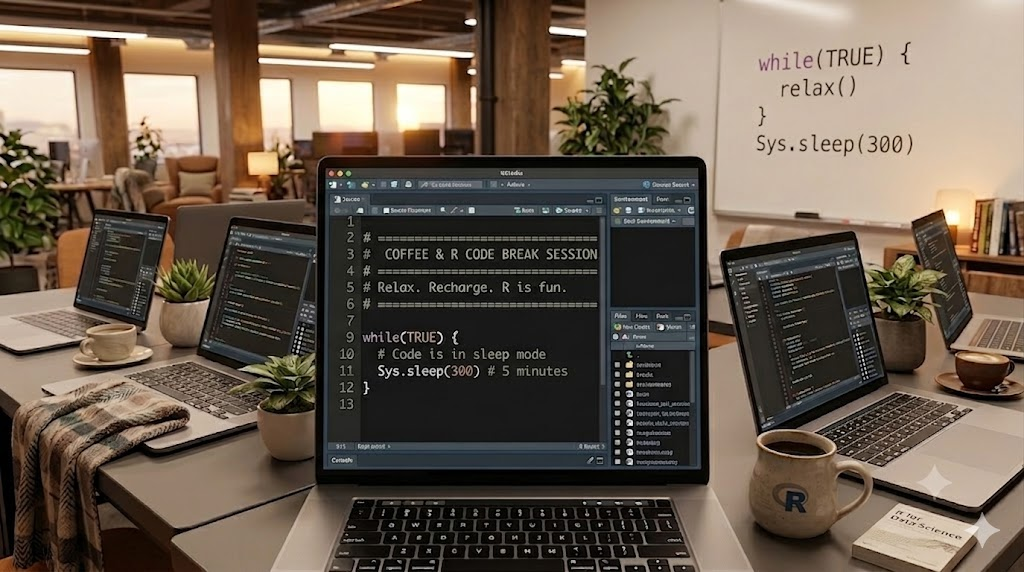
\includegraphics[keepaspectratio]{break.png}}
\end{frame}

\begin{frame}{Outline}
\protect\phantomsection\label{outline-1}
In this module, we will continue our discussion on Bootstrap.
\end{frame}

\begin{frame}{What is bootstrap?}
\protect\phantomsection\label{what-is-bootstrap}
A widely applicable, computer intensive resampling method used to
compute standard errors, confidence intervals, and significance tests.
\end{frame}

\begin{frame}{Why bootstrap?}
\protect\phantomsection\label{why-bootstrap}
\begin{itemize}
\tightlist
\item
  The exact sampling distribution of an estimator can be
  \textbf{difficult} to obtain
\item
  Asymptotic expansions are sometimes easier but expressions for
  standard errors based on large sample theory may not perform well in
  finite samples
\end{itemize}
\end{frame}

\begin{frame}{}
\protect\phantomsection\label{section}
\pandocbounded{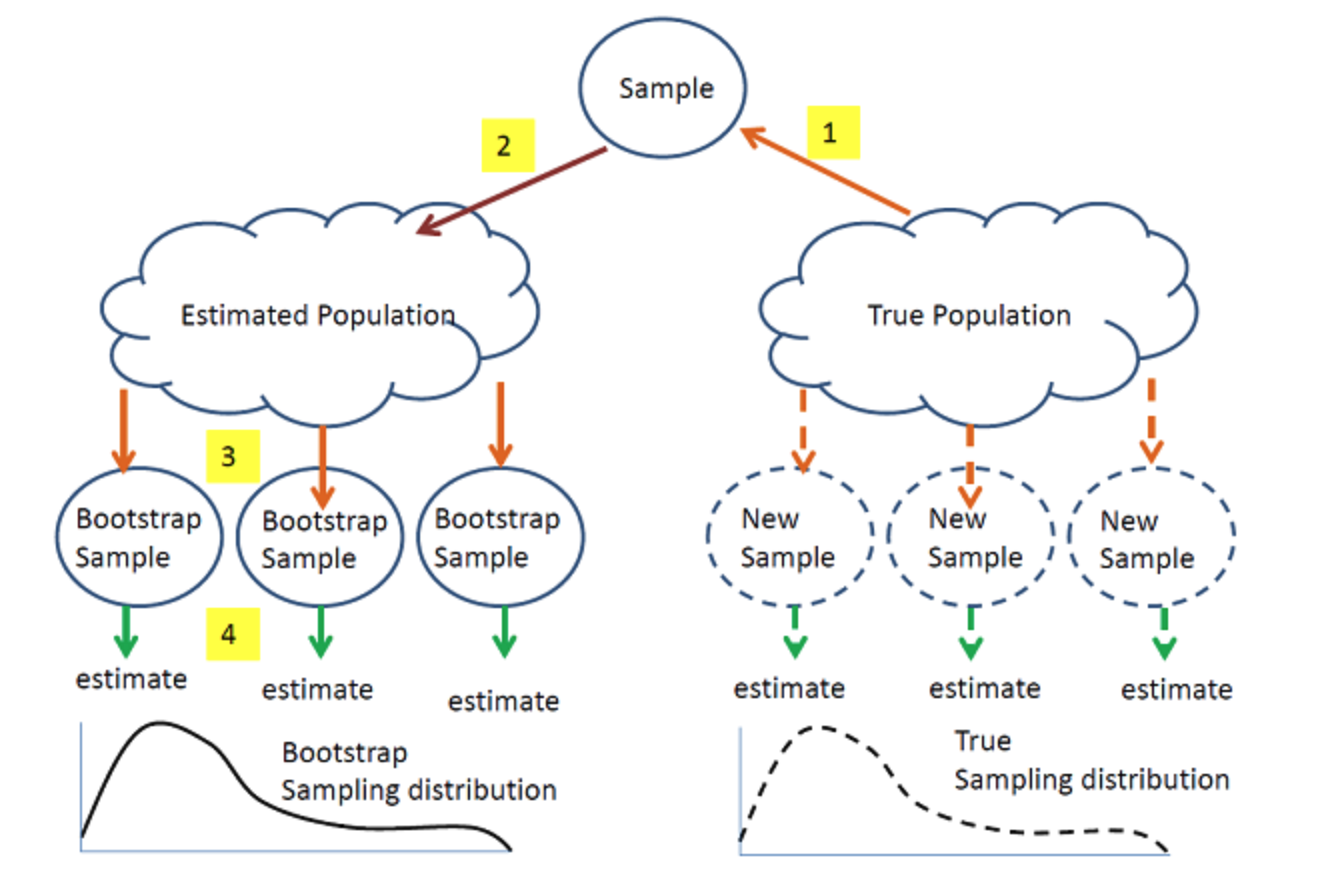
\includegraphics[keepaspectratio]{boot.png}}
\url{https://online.stat.psu.edu/stat555/node/119/}
\end{frame}

\begin{frame}{Example: estimate the variance of an estimator}
\protect\phantomsection\label{example-estimate-the-variance-of-an-estimator}
Now let \(\operatorname{Var}_F\left(T_n\right)\) denote the variance of
\(T_n\). The subscript \(F\) means the variance is a function of \(F\)
where \(F\) is the CDF of \(X\). If we know \(F\), we can directly
compute the variance. For example, if then \(x_1, \cdots, x_w\) iid \[
T_n=\bar{X}_n,=\frac{1}{n} \sum_{i=1}^n x_i
\] \[
\operatorname{Var}_F\left(T_n\right)=n^{-1}\left(\int x^2 d F(x)-\left(\int x d F(x)\right)^2\right)
\] which is a function of \(F\).
\end{frame}

\begin{frame}{Example: estimate the variance of an estimator}
\protect\phantomsection\label{example-estimate-the-variance-of-an-estimator-1}
When \(F\) is unknown, one can use an estimate of \(F\), e.g., the
empirical CDF \(\hat{F}_n\), i.e., \[
\hat{F}_n(x)=\frac{\sum_{i=1}^n \mathbf{1}\left(X_i \leq x\right)}{n} .
\] We then use a plug-in estimator for
\(\operatorname{Var}_{\hat{F}_n}\left(T_n\right)\) : \[
\operatorname{Var}_{\hat{F}_n}\left(T_n\right)=n^{-1}\left(\int x^2 d \hat{F}_n(x)-\left(\int x d \hat{F}_n(x)\right)^2\right) .
\]
\end{frame}

\begin{frame}{Example: estimate the variance of an estimator}
\protect\phantomsection\label{example-estimate-the-variance-of-an-estimator-2}
However, the plug-in estimator above can be hard to compute, we can then
approximate it with a simulation estimate, denoted by
\(V_{\text {boot }}\).

The following algorithm illustrate how one can do this through
bootstrap.

\begin{tabular}{l}
\hline Algorithm 1: Bootstrap variance estimation algorithm \\
\hline Input data $\left(X_1, \ldots, X_n\right) ;$ Number of iteration $B ;$ \\
for $i \leftarrow 0$ to $B$ do \\
$\quad \begin{array}{l}\text { Draw } X_{1, i}^*, \ldots, X_{n, i}^* \sim \hat{F}_n ; \\
\text { Compute } T_{n, i}^*=g\left(X_{1, i}^*, \ldots, X_{n, i}^*\right) ;\end{array}$ \\
end \\
$V_{\text {boot }}=\frac{1}{B} \sum_{i=1}^B\left(T_{n, i}^*-\frac{1}{B} \sum_{j=1}^B T_{n, j}^*\right)^2$. \\
\hline \end{tabular}

By law of large numbers, we have
\(V_{\text {boot }} \stackrel{\text { a.s. }}{\longrightarrow} \operatorname{Var}_{\hat{F}_n}\left(T_n\right)\)
as \(B \rightarrow \infty\).
\end{frame}

\begin{frame}{The bootstrap principle}
\protect\phantomsection\label{the-bootstrap-principle}
Suppose \(X=\left\{X_{1}, \ldots, X_{n}\right\}\) is a sample used to
estimate some parameter \(\theta=T(P)\) of the underlying distribution
\(P\). To make inference on \(\theta\), we are interested in the
properties of our estimator \(\hat{\theta}=S(X)\) for \(\theta\).

\pause

\begin{itemize}
\tightlist
\item
  If we knew \(P\),

  \begin{itemize}
  \tightlist
  \item
    we could obtain \(\left\{X^{b} \mid b=1, \ldots B\right\}\) from
    \(P\) and use Monte-Carlo to estimate the sampling distribution of
    \(\hat{\theta}\)
  \end{itemize}
\end{itemize}

\pause

\begin{itemize}
\tightlist
\item
  However, we don't,

  \begin{itemize}
  \tightlist
  \item
    we do the next best thing and resample from original sample,
    i.e.~the empirical distribution, \(\hat{P}\)
  \item
    we expect the empirical distribution to estimate the underlying
    distribution well by the \emph{Glivenko-Cantelli} Theorem
  \end{itemize}
\end{itemize}
\end{frame}

\begin{frame}{Why bootstrap works}
\protect\phantomsection\label{why-bootstrap-works}
Definition 2.1. Let \(F, G\) be two CDF's on a sample space \(X\). Let
\(\rho(F, G)\) be a metric on the space of CDF's on \(X\). We say
\(G_n^*\) is weakly \(\rho\)-consistent if \[
\rho\left(G_n^*, G_n\right) \stackrel{P}{\rightarrow} 0
\] as \(n \rightarrow \infty\). Similarly, \(G_n^*\) is strongly
\(\rho\)-consistent if \[
\rho\left(G_n^*, G_n\right) \stackrel{\text { a.s. }}{\longrightarrow} 0 .
\]
\end{frame}

\begin{frame}{Why bootstrap works}
\protect\phantomsection\label{why-bootstrap-works-1}
Now the measure of closeness between two CDF's depends on the metric
\(\rho\). The following two metrics are commonly used for the CDF's:

\begin{enumerate}
[(i)]
\item
  Kolmogorov metric: \[
  K(F, G)=\sup _{x \in R}|F(x)-G(x)| .
  \]
\item
  Mallows-Wasserstein metric: \[
  l_2(F, G)=\inf _{T_{F, G}}\left(E|Y-X|^2\right)^{1 / 2},
  \] where \(T_{F, G}\) is the collection of all possible joint
  distribution of the pair \((X, Y)\) whose marginal distributions are
  \(F, G\). The following theorem illustrates a special case of the
  bootstrap theory.
\end{enumerate}
\end{frame}

\begin{frame}{Why bootstrap works}
\protect\phantomsection\label{why-bootstrap-works-2}
Theorem. Suppose
\(X_1, \ldots, X_n \stackrel{\text { i.i.d. }}{\sim} F\) and
\(E\left(X_i^2\right)<\infty\). Let \[
T_n=g\left(X_1, \ldots, X_n\right)=\sqrt{n}(\bar{X}-\mu).
\] For the bootstrap version
\(T_n^* = \sqrt{n}(\bar{X}_n^* - \bar{X}_n)\): \[
K(G_n^*, G_n) \xrightarrow{a.s.} 0 \quad \text{and} \quad l_2(G_n^*, G_n) \xrightarrow{a.s.} 0
\] where: \begin{align*}
G_n(t) &= P(T_n \leq t) \quad \text{(True CDF)} \\
G_n^*(t) &= P(T_n^* \leq t \mid X_1, \dots, X_n) \quad \text{(Bootstrap CDF)}
\end{align*}
\end{frame}

\begin{frame}{Practical Implementation}
\protect\phantomsection\label{practical-implementation}
\begin{block}{Monte Carlo Approximation}
For finite samples, estimate $G_n^*$ via:
\[
\hat{G}_n^*(t) = \frac{1}{B}\sum_{b=1}^B \mathbb{I}(T_{n,b}^* \leq t)
\]
where:
\begin{itemize}
\item $B$ = number of bootstrap samples
\item $T_{n,b}^* = \sqrt{n}(\bar{X}_{n,b}^* - \bar{X}_n)$
\end{itemize}
\end{block}

\begin{exampleblock}{Convergence}
\begin{center}
\begin{tabular}{cc}
$B \to \infty$ & $\hat{G}_n^* \to G_n^*$ \\
$n \to \infty$ & $G_n^* \to G_n$ \\
\end{tabular}
\end{center}
\end{exampleblock}
\end{frame}

\begin{frame}{Bootstrap confidence intervals}
\protect\phantomsection\label{bootstrap-confidence-intervals}
For a statistic \(T_n\) with bootstrap replicates
\(\{T_{n,b}^*\}_{b=1}^B\):

\begin{itemize}
\item \textbf{Normal Approximation CI} (requires normality): \[
T_n \pm z_{\alpha/2}\widehat{se}_{boot}
\]
where $\widehat{se}_{boot}  = \sqrt{\frac{1}{B-1}\sum_{b=1}^B (T_{n,b}^* - \bar{T}^*)^2}$
\item \textbf{Pivotal (Basic) Bootstrap CI}:
\[
\Big(2T_n - T_{((1-\alpha/2)B)}^*, \ 2T_n - T_{((\alpha/2)B)}^*\Big)
\]

\item \textbf{Percentile Bootstrap CI}:
\[
\Big(T_{((\alpha/2)B)}^*, \ T_{((1-\alpha/2)B)}^*\Big)
\]
\end{itemize}
\end{frame}

\begin{frame}{Bootstrap confidence intervals}
\protect\phantomsection\label{bootstrap-confidence-intervals-1}
\begin{alertblock}{Important Notes}
\begin{itemize}
\item Normal CI assumes asymptotic normality of $T_n$
\item Pivotal CI inverts the bootstrap distribution
\item Percentile CI is simple but may be biased
\end{itemize}
\end{alertblock}
\end{frame}

\begin{frame}{Forms of bootstrap}
\protect\phantomsection\label{forms-of-bootstrap}
Based on how the population is estimated,

\begin{enumerate}
\tightlist
\item
  Nonparametric bootstrap
\item
  Parametric bootstrap
\item
  Empirical Bootstrap (Paired Bootstrap)
\item
  Residual Bootstrap
\item
  Wild Bootstrap
\end{enumerate}
\end{frame}

\begin{frame}{Nonparametric bootstrap (resampling)}
\protect\phantomsection\label{nonparametric-bootstrap-resampling}
\begin{block}{Core Idea}
Resample \textit{with replacement} from original data to approximate sampling distribution of statistic $\hat{\theta} = S(\mathbf{D})$
\end{block}

\pause
\begin{enumerate}
\item \textbf{Resampling}: Generate $B$ bootstrap datasets \\
$\mathbf{D}^*(1), \ldots, \mathbf{D}^*(B)$ where each $\mathbf{D}^*(b)$ contains $n$ observations drawn \textit{with replacement} from original data $\mathbf{D} = (X_1,\ldots,X_n)$

\pause
\item \textbf{Replication}: Compute bootstrap statistics \\
$\hat{\theta}^*(b) = S(\mathbf{D}^*(b))$ for $b=1,\ldots,B$

\pause
\item \textbf{Standard Error Estimation}:
\[
\widehat{se}_{boot} = \sqrt{\frac{1}{B-1}\sum_{b=1}^B \left(\hat{\theta}^*(b) - \bar{\theta}^*\right)^2}
\]
where $\bar{\theta}^* = \frac{1}{B}\sum_{b=1}^B \hat{\theta}^*(b)$
\end{enumerate}
\end{frame}

\begin{frame}{Parametric bootstrap}
\protect\phantomsection\label{parametric-bootstrap}
\begin{itemize}
\item
  Assumes the data comes from a known distribution with unknown
  parameters
\item
  First estimate the parameters from the data and then use the estimated
  distribution to simulate the samples
\end{itemize}
\end{frame}

\begin{frame}{Bootstrap for Regression}
\protect\phantomsection\label{bootstrap-for-regression}
Bootstrap can also be used to conduct statistical inference for
regression model. Let
\(\left(X_1, Y_1\right), \ldots,\left(X_n, Y_n\right)\) be the observed
data and \[
E\left(Y_i \mid X_i=x\right)=\beta_0+\beta_1 x,
\] i.e., \[
Y_i=\beta_0+\beta_1 X_i+\epsilon_i .
\] There are several variants to the bootstrap under regression setting.
\end{frame}

\begin{frame}{Empirical Bootstrap (Paired Bootstrap)}
\protect\phantomsection\label{empirical-bootstrap-paired-bootstrap}
We generate a new sets of i.i.d. observations
\(\left(X_1^*, Y_1^*\right), \ldots,\left(X_n^*, Y_n^*\right)\) such
that for each \(l\), \[
P\left(X_l^*=X_i, Y_l^*=Y_i\right)=\frac{1}{n}
\] for all \(i\). Similar to bootstrap estimation of variance, we repeat
this procedure \(B\) times and fit a linear regression model for each of
the generated paired data: \[
\begin{gathered}
\left(X_1^{*(1)}, Y_1^{*(1)}\right), \ldots,\left(X_n^{*(1)}, Y_n^{*(1)}\right) \stackrel{\text { fit linear regression }}{\longrightarrow} \hat{\beta}_0^{*(1)}, \hat{\beta}_1^{*(1)} \\
\ldots \\
\left(X_1^{*(B)}, Y_1^{*(B)}\right), \ldots,\left(X_n^{*(B)}, Y_n^{*(B)}\right) \stackrel{\text { fit linear regression }}{\longrightarrow} \hat{\beta}_0^{*(B)}, \hat{\beta}_1^{*(B)} .
\end{gathered}
\]
\end{frame}

\begin{frame}{Empirical Bootstrap (Paired Bootstrap)}
\protect\phantomsection\label{empirical-bootstrap-paired-bootstrap-1}
We then estimate the bootstrap variance \[
\hat{\operatorname{Var}}\left(\hat{\beta}_0\right)=\frac{1}{B} \sum_{l=1}^B\left(\hat{\beta}_0^{*(l)}-\bar{\beta}_0^*\right)^2, \bar{\beta}_0^*=\frac{1}{B} \sum_{i=1}^B \hat{\beta}_0^{*(l)},
\] and \[
\hat{\operatorname{Var}}\left(\hat{\beta}_1\right)=\frac{1}{B} \sum_{l=1}^B\left(\hat{\beta}_1^{*(l)}-\bar{\beta}_1^*\right)^2, \bar{\beta}_1^*=\frac{1}{B} \sum_{l=1}^B \hat{\beta}_1^{*(l)} .
\] We can also obtain the bootstrap CI as \[
\hat{\beta}_0 \pm z_{1-\alpha / 2} \sqrt{\hat{\operatorname{Var}}\left(\hat{\beta}_0\right)}
\] and \[
\hat{\beta}_1 \pm z_{1-\alpha / 2} \sqrt{\hat{\operatorname{Var}}\left(\hat{\beta}_1\right)}
\]
\end{frame}

\begin{frame}{Empirical Bootstrap (Paired Bootstrap)}
\protect\phantomsection\label{empirical-bootstrap-paired-bootstrap-2}
Although empirical bootstrap works well in practice, it may lead to a
bad results, especially in the presence of influential observations
(some \(X_i\) 's are very far away from the others).

This will also strongly affect the empirical bootstrap in the sense that
if an empirical bootstrap does not select these influential points, the
regression coefficients can be very different.
\end{frame}

\begin{frame}{Residual Bootstrap}
\protect\phantomsection\label{residual-bootstrap}
To solve the problem of empirical bootstrap illustrated previously, we
may use the residual bootstrap. We first fit the original data to obtain
the OLS estimate \(\hat{\beta}_0, \hat{\beta}_1\). Define \[
e_i=Y_i-\hat{Y}_i=Y_i-\hat{\beta}_0-\hat{\beta}_1 X_i .
\] \(e_i\) here are the fitted residuals and can be regarded as a good
approximation of \(\epsilon_i\). The residual bootstrap generate i.i.d.
\(\hat{\epsilon}_1^*, \ldots, \hat{\epsilon}_n^*\) such that for each
\(\hat{\epsilon}_l^*\), \[
P\left(\hat{\epsilon}_l^*=e_i\right)=\frac{1}{n} .
\] Then we generate a new bootstrap sample \[
\left(X_1^*, Y_1^*\right), \ldots,\left(X_n^*, Y_n^*\right)
\] via \[
X_i^*=X_i, Y_i^*=\hat{\beta}_0+\hat{\beta}_1 X_i+\hat{\epsilon}_i^* .
\]
\end{frame}

\begin{frame}{Wild Bootstrap}
\protect\phantomsection\label{wild-bootstrap}
Another issue usually occur in linear regression is the so called
phenomenon of heteroskedasticity, i.e.,
\(\operatorname{Var}\left(\epsilon_i \mid X_i\right)\) depends on the
value of \(X_i\).

Now residual bootstrap cannot deal with this issue. In particular, the
residual bootstrap will be unstable because the residual bootstrap will
swap all the residuals regardless of the value of the covariate. The
solution to this is through the wild bootstrap.

The wild bootstrap first generate i.i.d. random variables
\(V_1, \ldots, V_n \sim \mathcal{N}(0,1)\) and then generate the
bootstrap sample \[
\left(X_1^*, Y_1^*\right), \ldots,\left(X_n^*, Y_n^*\right)
\] by \[
Y_i^*=\hat{\beta}_0+\hat{\beta}_1 X_i+V_i e_i, X_i^*=X_i .
\]
\end{frame}

\begin{frame}[fragile]{Bootstrap hypothesis testing}
\protect\phantomsection\label{bootstrap-hypothesis-testing}
\tiny

\begin{Shaded}
\begin{Highlighting}[]
\NormalTok{boot\_dat }\OtherTok{\textless{}{-}} \ControlFlowTok{function}\NormalTok{(x, n, mu, std) \{}
\NormalTok{  newx }\OtherTok{\textless{}{-}} \FunctionTok{sample}\NormalTok{(x, n, }\AttributeTok{replace =}\NormalTok{ T)}
  \FunctionTok{return}\NormalTok{((}\FunctionTok{mean}\NormalTok{(newx) }\SpecialCharTok{{-}}\NormalTok{ mu)}\SpecialCharTok{/}\NormalTok{(std}\SpecialCharTok{/}\FunctionTok{sqrt}\NormalTok{(n)))}
\NormalTok{\}}


\NormalTok{pvalues\_1 }\OtherTok{\textless{}{-}} \FunctionTok{rep}\NormalTok{(}\ConstantTok{NA}\NormalTok{, nsim)}
\NormalTok{pvalues\_2 }\OtherTok{\textless{}{-}} \FunctionTok{rep}\NormalTok{(}\ConstantTok{NA}\NormalTok{, nsim)}

\ControlFlowTok{for}\NormalTok{ (i }\ControlFlowTok{in} \DecValTok{1}\SpecialCharTok{:}\NormalTok{nsim)\{}
\NormalTok{  x }\OtherTok{\textless{}{-}} \FunctionTok{rnorm}\NormalTok{(n, }\AttributeTok{mean =}\NormalTok{ mu, }\AttributeTok{sd =}\NormalTok{ std)}
\NormalTok{  stat }\OtherTok{\textless{}{-}} \FunctionTok{abs}\NormalTok{((}\FunctionTok{mean}\NormalTok{(x) }\SpecialCharTok{{-}}\NormalTok{ mu)}\SpecialCharTok{/}\NormalTok{(std}\SpecialCharTok{/}\FunctionTok{sqrt}\NormalTok{(n)))}
\NormalTok{  pvalues\_1[i] }\OtherTok{\textless{}{-}} \DecValTok{2}\SpecialCharTok{*}\NormalTok{(}\DecValTok{1} \SpecialCharTok{{-}} \FunctionTok{pnorm}\NormalTok{(stat))}
  
  
\NormalTok{  newx }\OtherTok{\textless{}{-}}\NormalTok{ x }\SpecialCharTok{{-}} \FunctionTok{mean}\NormalTok{(x) }\SpecialCharTok{+}\NormalTok{ mu}
\NormalTok{  boot\_scores }\OtherTok{\textless{}{-}} \FunctionTok{sapply}\NormalTok{(}\DecValTok{1}\SpecialCharTok{:}\NormalTok{nboot, }
                        \ControlFlowTok{function}\NormalTok{(index) }\FunctionTok{boot\_dat}\NormalTok{(newx, n, mu, std))}
\NormalTok{  boot\_scores }\OtherTok{\textless{}{-}} \FunctionTok{as.vector}\NormalTok{(boot\_scores)}
  \CommentTok{\# hist(boot\_scores)}
  \CommentTok{\# mean(boot\_scores)}
\NormalTok{  pvalues\_2[i] }\OtherTok{\textless{}{-}} \FunctionTok{length}\NormalTok{(}\FunctionTok{which}\NormalTok{(boot\_scores }\SpecialCharTok{\textgreater{}}\NormalTok{ stat))}\SpecialCharTok{/}\FunctionTok{length}\NormalTok{(boot\_scores) }\SpecialCharTok{+} 
    \FunctionTok{length}\NormalTok{(}\FunctionTok{which}\NormalTok{(boot\_scores }\SpecialCharTok{\textless{}}\NormalTok{ (}\SpecialCharTok{{-}}\NormalTok{stat)))}\SpecialCharTok{/}\FunctionTok{length}\NormalTok{(boot\_scores)}
\NormalTok{\}}
\end{Highlighting}
\end{Shaded}
\end{frame}

\begin{frame}{Failures of Bootstrap}
\protect\phantomsection\label{failures-of-bootstrap}
Let \(X_1, \ldots, X_n \stackrel{\text { i.i.d. }}{\sim}\) unif
\((0,1)\) and \(M_n=\min \left(X_1, \ldots, X_n\right)\) be the minimum
of the sample. One can show that \[
n M_n \stackrel{\mathcal{D}}{\rightarrow} \exp (1)
\] However, let \(M_n^*=\min \left(X_1^*, \ldots, X_n^*\right)\) be the
minimum of a bootstrap sample, then \[
P\left(\text { none of } X_1^*, \ldots, X_n^* \text { select } M_n\right)=\left(1-\frac{1}{n}\right)^n \approx e^{-1},
\] which implies that \[
P\left(M_n^*=M_n\right) \approx 1-e^{-1} .
\] Therefore, \(M_n^*\) has a huge probability mass at \(M_n\). This
means the distribution of \(M_n^*\) is very different from the
distribution of \(M_n\). The detailed proof is left as homework.
\end{frame}

\begin{frame}{StatQuest videos}
\protect\phantomsection\label{statquest-videos}
Check out these videos made by Josh Starmer with vivid illustration for
the boostrap!

\begin{itemize}
\item
  Bootstrapping Main Ideas
  {[}\href{https://youtu.be/Xz0x-8-cgaQ}{link}{]}
\item
  Using Bootstrapping to Calculate p-values
  {[}\href{https://youtu.be/N4ZQQqyIf6k}{link}{]}
\end{itemize}
\end{frame}

\begin{frame}{Resources}
\protect\phantomsection\label{resources}
This tutorial is based on

\begin{itemize}
\item
  PennState STAT555 Statistical Analysis of Genomics Data
  {[}\href{https://online.stat.psu.edu/stat555/node/119/}{links}{]}.
\item
  Harvard's Biostatistics Preparatory Course Methods
  {[}\href{https://isabelfulcher.github.io/methodsprep/slides/Lecture_7/2018_Lecture_07.pdf}{links}{]}.
\end{itemize}
\end{frame}

\end{document}
